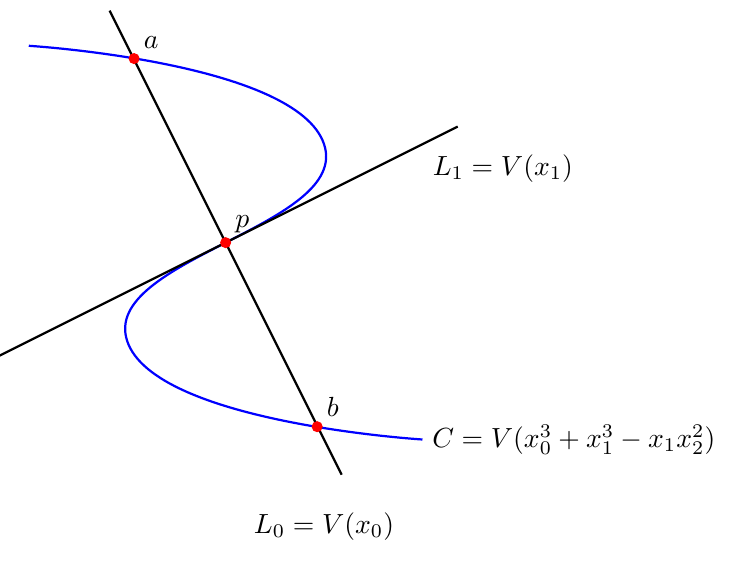
\begin{tikzpicture}[scale=1.25]
  \draw[blue, thick, smooth, tension=1] plot coordinates{
    (2,-2)
    (-1, -1)
    (1,1)
    (-2, 2)
  };
  \draw (2,-2) node [right] {$C = V(x_0^3+x_1^3-x_1x_2^2)$};
  \draw[shorten >=-0.5cm, shorten <=-0.5cm, thick] (-2,-1) -- (2,1) node [below right] {$L_1 = V(x_1)$};
  \draw[shorten >=-0.5cm, shorten <=-0.5cm, thick] (-1,2) -- (1,-2) node [below=0.8cm] {$L_0 = V(x_0)$};
  \draw[red, fill] (0,0) circle (0.05) node [black, above right] {$p$};
  \draw[red, fill] (-0.93, 1.87) circle (0.05) node [black, above right] {$a$};
  \draw[red, fill] (0.93, -1.87) circle (0.05) node [black, above right] {$b$};
\end{tikzpicture}

%%% Local Variables:
%%% mode: latex
%%% TeX-master: "../main"
%%% End:
